\section{Growth stages through late times} \slabel{late}

\begin{figure*}
\begin{subfigure}[b]{\columnwidth}
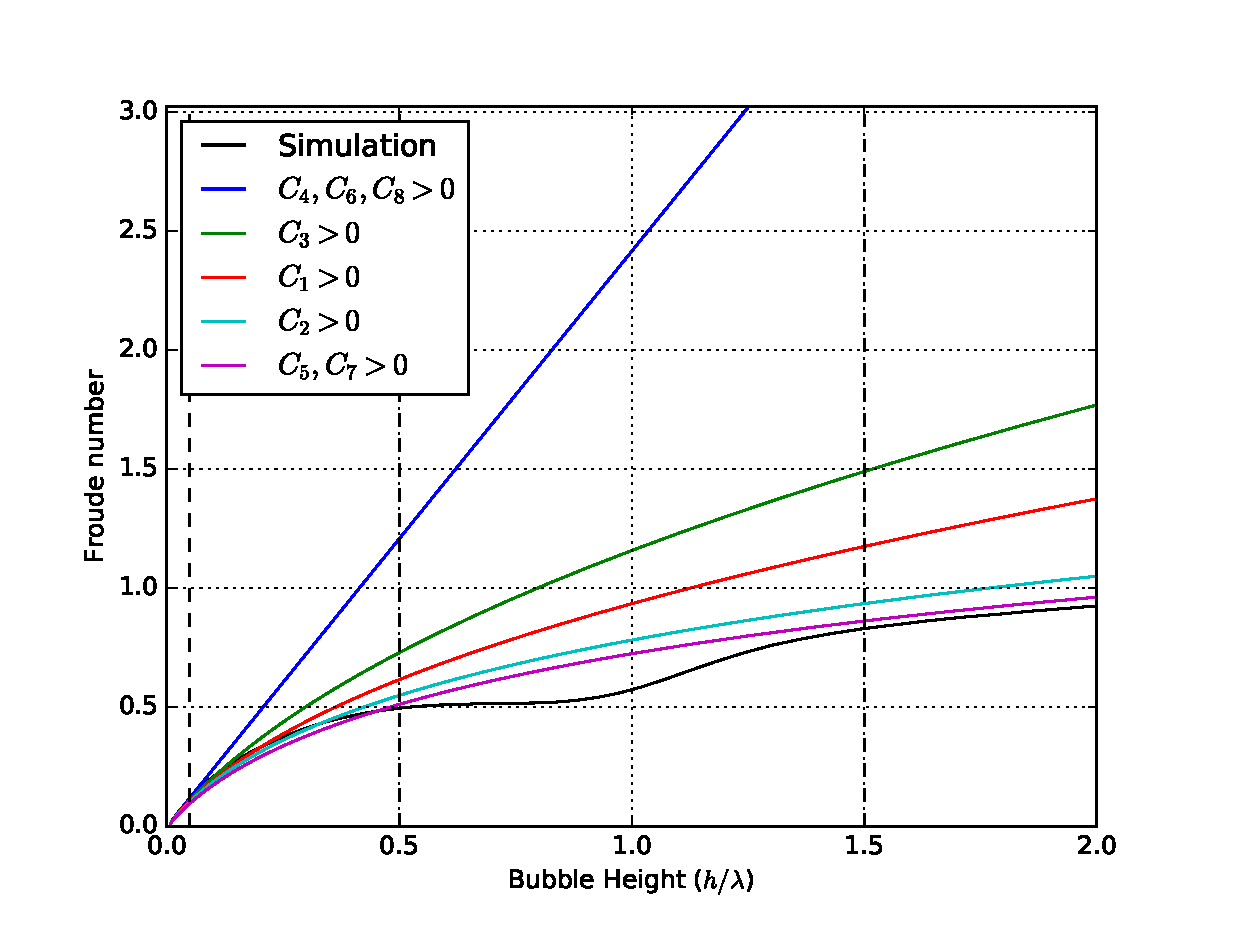
\includegraphics[width=\columnwidth]{figs/Cascade-short-4-1}
\caption{Early times}
\end{subfigure}
\begin{subfigure}[b]{\columnwidth}
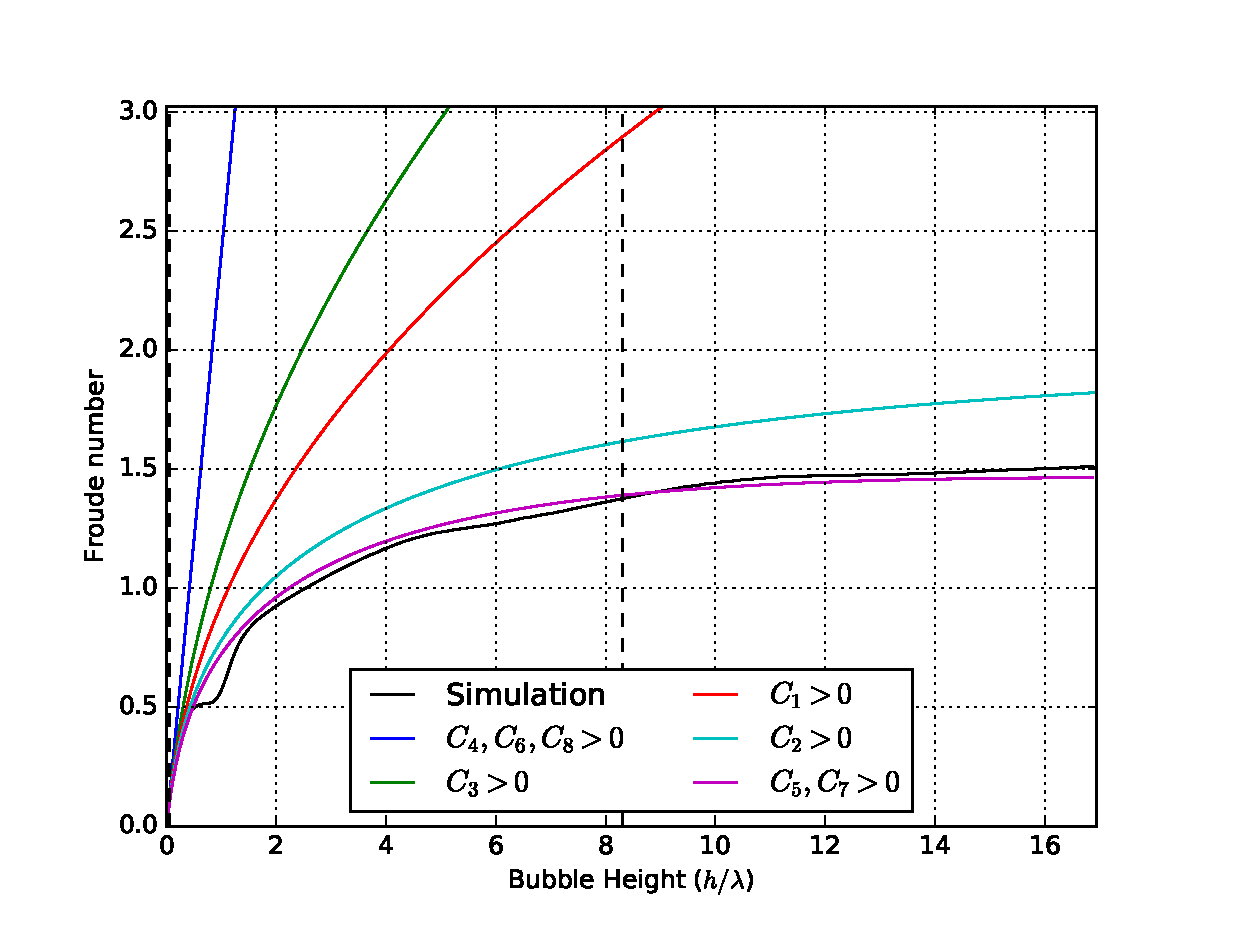
\includegraphics[width=\columnwidth]{figs/Cascade-4-1}
\caption{Late times}
\end{subfigure}
\caption{ \flabel{high_Ra_traj}
Bubble Froude number vs non-dimensional bubble height for $\text{Ra} = 10^{5.75}, \text{Sc} = 4$, simulation vs model with successive terms enabled.
The dashed vertical lines divide the trajectory into four regimes: linear growth for $H/\lambda < .05$, saturation until $H / \lambda = 0.5$, stagnation and re-acceleration until $H / \lambda = 1.5$, and dissipation beyond that.
}
\end{figure*}

\begin{figure*}
\begin{subfigure}[b]{\columnwidth}
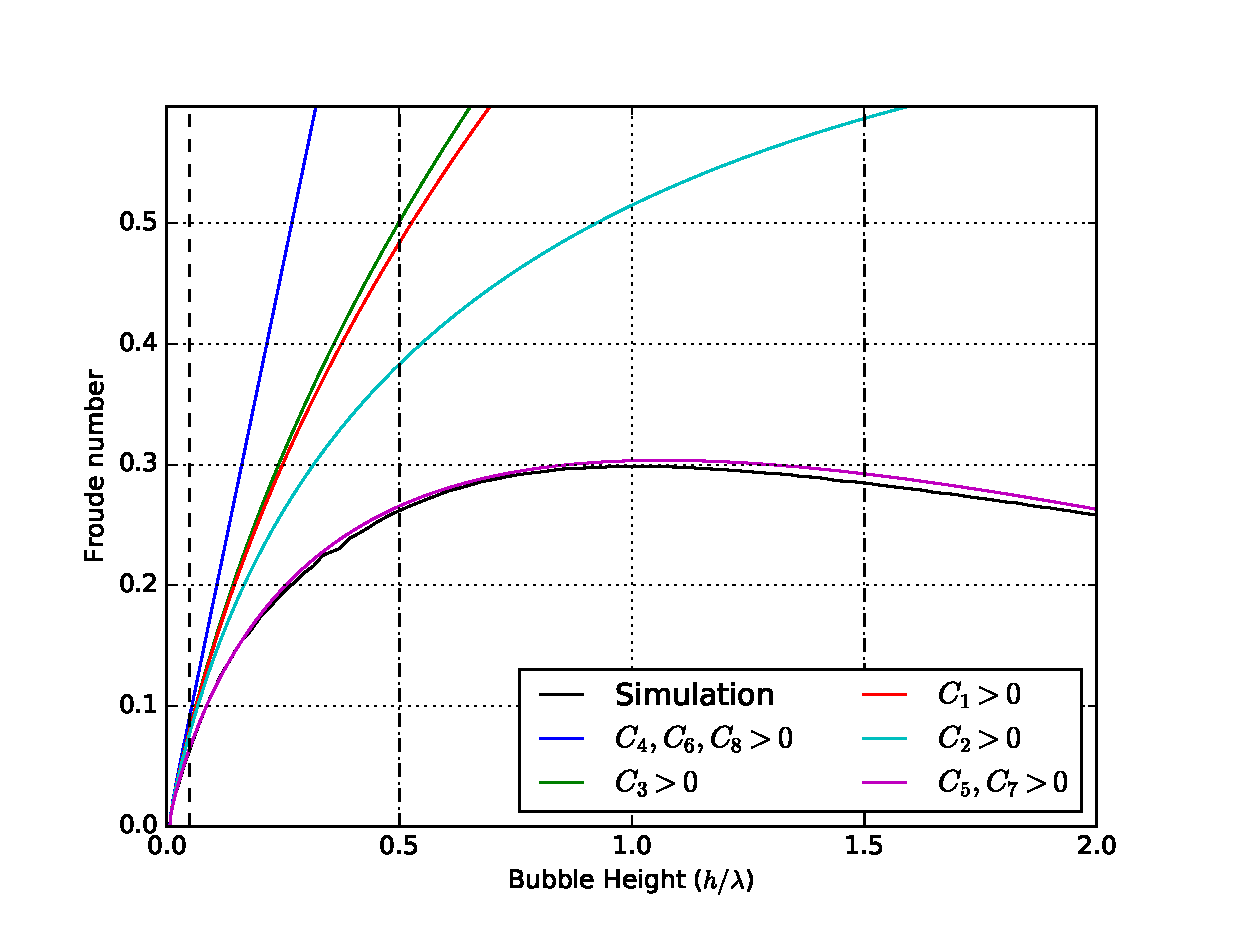
\includegraphics[width=\columnwidth]{figs/Cascade-short-32-4}
\caption{Early times}
\end{subfigure}
\begin{subfigure}[b]{\columnwidth}
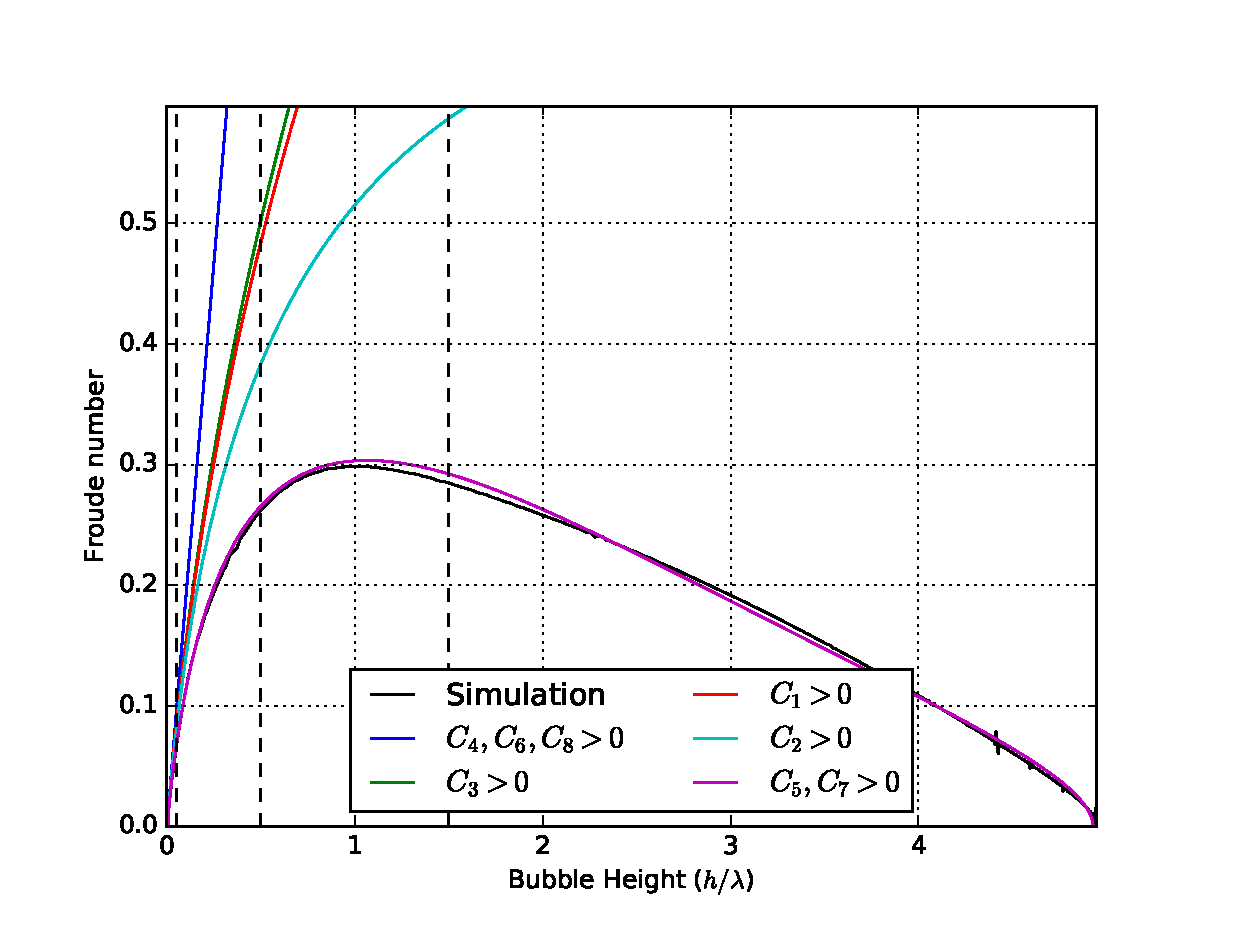
\includegraphics[width=\columnwidth]{figs/Cascade-32-4}
\caption{Late times}
\end{subfigure}
\caption{ \flabel{low_Ra_traj}
Bubble Froude number vs non-dimensional bubble height for $\text{Ra} = 10^{4.5}, \text{Sc} = 8$, simulation vs model with successive terms enabled.
Dashed vertical lines divide the trajectory, as in \fref{high_Ra_traj}, but the saturation regime and stagnation and re-acceleration regime are suppressed by mixing.
}
\end{figure*}

Single mode experiments have been limited to bubble heights of $1.8\lambda$~\cite{Wilkinson2007}.
Simulations have reached in $4\lambda$ in 3D~\cite{Ramaprabhu2012} and $9\lambda$ in 2D~\cite{Wei2012}.
Here, we present trajectories that continue up to $17\lambda$, e.g. \fref{high_Ra_traj}.
However, the low Rayleigh number bubbles stop rising at lower aspect rations, e.g. \fref{high_Ra_traj}.

In the spirit of recent analyses~\cite{Ramaprabhu2012, Wei2012}, we try to identify distinct growth regimes.
To do so, we consider the behavior of the simple model with coefficients set to zero.
Initially, only $C_4$, $C_6$, and $C_8$ affect bubble dynamics.
The growth is exponential with a rate in agreement with the linear theory, so we term this the linear regime.
As the bubble grows, the $C_3$ term reduces the growth rate to a limiting value of $A g / C_3$.
Because this represents the transition from exponential growth to free-fall, we term it the saturation regime.
The $C_1$ term has the same qualitative effect as the $C_3$ term, so it doesn't distinguish a unique regime.
The $C_2$ term does impose a limiting velocity scale, so it departs significantly from the $C_3$ dynamics in the viscous regime.
Finally, the $C_5$ term, balanced by the $C_7$ term, mix the fluid and reduce the effective Atwood number in the diffusive regime.
Because the relative onset of the viscous and diffusive regimes depends on the Schmidt number, they are grouped together into the dissipative regime.
Ultimately, the bubble stops rising.
The bubble height at this point, which is also the maximum bubble height, is called the penetration depth.

\subsection{Exponential growth}
When the amplitude is small and the interface is thin, the linear theory and numerical results identify exponential growth: $\ddot{h} = \gamma^2 h$.
Similarly, in the limit $h, \delta \rightarrow 0$, the simple model yields a growth rate:
\begin{equation}
\gamma = \sqrt{\frac{A_0 g k}{2 \pi C_4(1 + C_8 / C_6 \pi^{1/2} k \delta)}},
\end{equation}
which differs from the linear theory by the absence of a $-D k^2$ term.
This is the only term that can cause unstable interfaces to decay, i.e. $\gamma < 0$ for positive Atwood numbers.
In the simple model, all unmixed bubbles grow while in the linear theory highly diffusive bubbles decay.

The other terms, i.e. those scaled by $C_1, C_2, C_3, C_5$ and $C_7$, can be omitted while the description of the exponential growth is unaffected.

\subsection{Saturation regime}
The exponential growth saturates as the bubble height increases.
In the simple model, this captured by the $C_3$ term:
\begin{equation}
\ddot{h} = \frac{A g}{(C_3 h + C_4 \lambda) (1 + C_8 / C_6 \pi^{1/2} k \delta)},
\end{equation}
which becomes significant when $h \approx C_4 \lambda / C_3$.
We will find in the following section that $C_3$ takes a value of about 1, so, omitting viscous corrections, saturation halves the growth rate at $h \approx \lambda / (2\pi)$.

The definition of the start of the saturation regime is somewhat arbitrary.
Here, we propose the definition $h/\lambda < 0.05$ as it is where the exponential and saturated plots of the Froude number vs height visually deviate.
The important thing is that this threshold is independent of $Ag$, the Grashof number, and the Rayleigh number.
Within the saturation regime, the acceleration takes a limiting value of $Ag$, defining a saturation velocity:
\begin{equation} \elabel{vel_sat}
v_s \sim \sqrt{A g h}
\end{equation}

\subsection{Viscous regime}
As the bubble grows, so does its surface area.
The viscous drag, which scales linearly with the bubble height and bubble velocity, ultimately balances the buoyancy to limit the velocity, as in \eref{visc_vel}.
The scaling of the onset of this regime can be found by equating the saturation velocity and the viscous velocity:
\begin{equation}
\sqrt{A g h} \sim \frac{A g \lambda^2}{\nu}.
\end{equation}
Solving for $h/\lambda$ yields:
\begin{equation}
\frac{h_\nu}{\lambda} \sim \frac{A g \lambda^3}{\nu^2} = \text{Gr},
\end{equation}
where $h_\nu$ is the onset of the viscous regime.

As in the saturation case, the particular definition of the onset is arbitrary.
Here, we will define $h_\nu$ such that when $h_\nu/\lambda = 1$, the viscous velocity has the potential flow value: $v_\nu = \pi^{-1/2} \sqrt{A g \lambda}$.
This works out to be:
\begin{equation}
\frac{h_\nu}{\lambda} = \frac{\pi}{C_2^2} \text{Gr} \approx 2.4 \times 10^{-4} \text{Gr}
\end{equation}

\subsection{Diffusive regime}
\begin{figure}
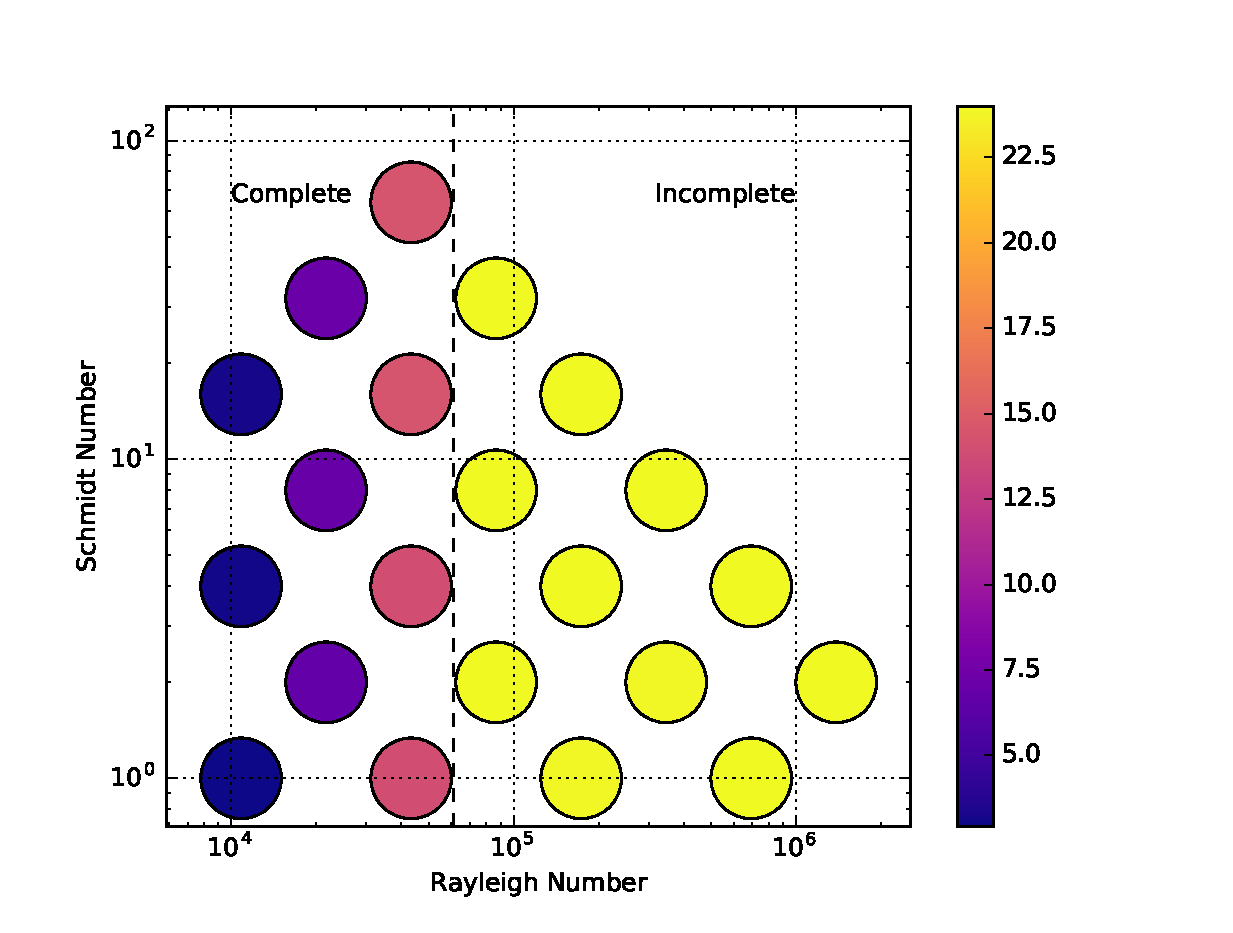
\includegraphics[width=\columnwidth]{figs/PenetrationDepth-vs-Rayleigh-Schmidt}
\caption{ \flabel{depth_scatter}
  Penetration depth, non-dimensionalized, vs the Rayleigh and Schmidt numbers.
  The dashed line separates completed from incomplete trajectories, which are clipped at $h/\lambda \approx 23$.
}
\end{figure}

\begin{figure}
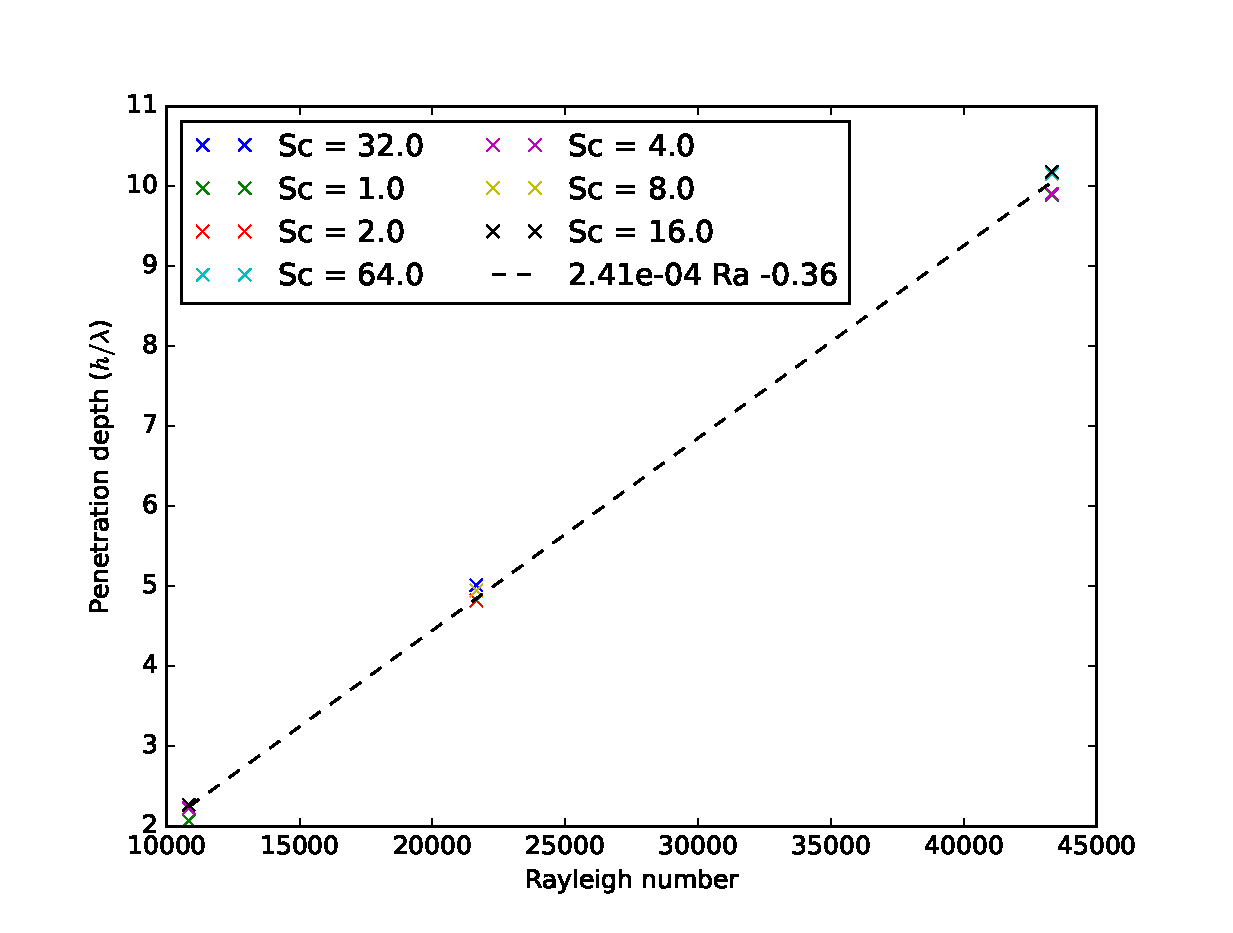
\includegraphics[width=\columnwidth]{figs/Depth-vs-Rayleigh}
\caption{ \flabel{depth_line}
  Penetration depth, non-dimensionalized, vs the Rayleigh.
  The dashed line is a best fit line.
}
\end{figure}

The rate of diffusion across the surface of the bubble also scales with the bubble height.
When the viscous drag limits the bubble's velocity, the flux of pure fluid into the bubble, which goes as the velocity, is unable to match the flux of mixed fluid through the interface.
Mixing dilutes the buoyant fluid, reducing the Atwood number and therefore the bubble velocity.
Ultimately, the Atwood number reaches zero and the bubble stops rising.

The penetration depth is the maximum height of the bubble, which is the height of the bubble at the stopping condition of this analysis.
We can estimate the scaling of the penetration depth as the product of a characteristic velocity with a characteristic time-scale.
The late-time velocity is the viscous velocity, $v_\nu$, while time-scale is given by diffusion:
\begin{equation}
\tau_D = \frac{\lambda^2}{D}.
\end{equation}
Combining and non-dimensionalizing yields:
\begin{equation}
\frac{h(\infty)}{\lambda} = \frac{A g \lambda^3}{\nu D} = \text{Ra},
\end{equation}
so the penetration depth should go linearly with the Rayleigh number.

The penetration depth is plotted as a function of Rayleigh and Schmidt number in \fref{depth_scatter}, and, indeed, depends strongly on the Rayleigh number before being clipped by the top walls.
Furthermore, the relationship to the Rayleigh number is linear over the cases shown here, as shown in \fref{depth_line}.

\subsection{Stagnation and re-acceleration}

Absent from the previous discussion is the stagnation and re-acceleration of the bubble around $h / \lambda = 1$, as seen in \fref{high_Ra_traj}.
There are no terms in the buoyancy-drag model capable of producing an inflection point in the Froude number vs bubble height, so stagnation and re-acceleration cannot be controlled by turning a model coefficient on or off.
This suggests that the buoyancy-drag model is missing a term.

However, the buoyancy-drag model does have a limiting velocity, the viscous velocity $v_\nu$.
When the viscous velocity is near or below the stagnation velocity, $\text{Fr} \approx \pi^{-1/2}$, saturation and re-acceleration are suppressed.
Otherwise, stagnation and re-acceleration temporarily interrupt the saturation regime.
The stagnation and re-acceleration is a transient regime that only occurs at sufficiently high Grashof numbers.

